

%%%%%%%%%%%%%%%%%%%%%%%%%%%%%%%%%%%%%%%%%%%%%%%%%%%%%%%%%%%%%
%%%%%%%%%%%%%%%%%%%%%%%%%%%%%%%%%%%%%%%%%%%%%%%%%%%%%%%%%%%%%
%
%  %%%%%%%  %    %  %%%%%%  %%%%%%  %%%%%%%  %%%%%%%  %%%%%
%  %        %    %  %    %  %     %    %     %        %    %
%  %        %    %  %%%%%%  %     %    %     %        %    %
%  %        %%%%%%  %    %  %%%%%%     %     %%%%%    %%%%%
%  %        %    %  %    %  %          %     %        %    %
%  %%%%%%%  %    %  %    %  %          %     %%%%%%%  %     %
%
%%%%%%%%%%%%%%%%%%%%%%%%%%%%%%%%%%%%%%%%%%%%%%%%%%%%%%%%%%%%%
%%%%%%%%%%%%%%%%%%%%%%%%%%%%%%%%%%%%%%%%%%%%%%%%%%%%%%%%%%%%%

\chapter{The Theory of Sheaves and Cosheaves}
\label{sec:abstract_sheaves}

\begin{quote}
{\em ``Nous nous proposons d'indiquer sommairement comment les m\'ethodes par lesquelles nous avons etudi\'e la topologie d'un espace peuvent \^{e}tre adapt\'ees \`a l'\'etude de la topologie d'une repr\'esentation.''}\footnote{``We propose to state briefly how the methods by which we have studied the topology of a space can be adapted to the study of the topology of maps.''}
\begin{flushright} --- Jean Leray~\cite{leray46representation} \end{flushright}
\end{quote}

In its most general form, the subject of this thesis involves the assignment of data to subsets of a space $X$. This should sound like a very useful thing to do. After all, we have in both pure and applied mathematics many an occasion to record data or solutions in a local, spatially distributed way. Immediate questions arise: To which subsets should we assign data? What should these assignments be used for? What are they to be called?

The author believes such assignments are to be called sheaves or cosheaves depending on whether it is natural to restrict data from larger spaces to smaller spaces or by extending data from smaller spaces to larger ones. The evolution of these ideas deserves some discussion and the eager historian should consult John Gray's ``Fragments of the History of Sheaf Theory,''~\cite{gray} for a more thorough account. However, we outline three basic opinions on what a sheaf (or cosheaf) is really:
\begin{itemize}\index{sheaf!three perspectives on}\index{cosheaf!three perspectives on}
	\item A sheaf is a \textbf{system of coefficients} for computing cohomology that weighs and measures parts of the space differently. A cosheaf, in like manner, is a system of coefficients for homology that varies throughout the space.
	\item A sheaf is an \textbf{\'etal\'e space} $E$ along with a local homeomorphism $\pi:E\to X$. Analogously, a cosheaf is a locally-connected space $D$, called the \textbf{display locale}, that maps to $X$~\cite{funk-display}.
	\item A sheaf (or a cosheaf) is an \textbf{abstract assignment of data} --- a functor --- that further satisfies a gluing axiom expressed by limits (or colimits).
\end{itemize}

Historically, the system of coefficients perspective came first. In a 1943 paper Norman Steenrod defined a new homology theory determined by assigning abelian groups directly to \emph{points} of a space $X$ and group isomorphisms to (homotopy classes of) paths between points~\cite{steenrod}. This theory was vastly generalized in 1946 by Jean Leray where a \textbf{faisceau} (or sheaf) was defined to be a way of assigning modules to \emph{closed sets} in an inclusion-reversing way.\index{sheaf!on closed sets}
\[
	\xymatrix{V \ar[rr] \ar[rd] & & X \\ & W \ar[ru] &} \qquad \qquad \qquad \xymatrix{F(V) & & \ar[ll] \ar[ld] F(X) \\ & F(W) \ar[lu] &}
\]
Although this strengthened the abstract assignment perspective, Leray was still concerned with the cohomological ideas developed by Georges de Rham, Kurt Reidemeister and Hassler Whitney. 

By the early 1950s, Henri Cartan and his seminar revised Leray's definition of a sheaf to consist of a local homeomorphism $\pi:E\to X$. One could re-obtain the assignment perspective by attaching to each \emph{open set} $U$ the set of sections of this map over $U$: 
\[
	U \rightsquigarrow \{s:U\to E\, |\, \pi\circ s(x)=x\}
\]
One plausible explanation for using open sets is provided by the \textbf{open pasting lemma}, which states\footnote{Munkres calls this the ``local formulation of continuity'' in theorem 18.2(f)~\cite{munkres}. Munkres reserves the term ``pasting lemma'' for the closed set version, which is stated directly afterwards as theorem 18.3.} that if $X=\cup U_i$ is a (potentially infinite) union of open sets equipped with continuous sections $s_i:U_i\to E$ that agree on overlaps, then the set-theoretically defined section $s:X\to E$ will also be continuous. If closed sets are used, then this gluing argument only works for covers consisting of finitely many closed sets.

Finally, the Weil conjectures in algebraic geometry motivated the introduction of a more general notion of a topology and cohomology. Following suggestions of Jean-Pierre Serre, the domain of a sheaf was abstracted by Alexander Grothendieck from subsets $U\subseteq X$ to collections of mappings $U\to X$ that satisfy certain conditions reminiscent of an open cover~\cite{mm-topos}. Defining a sheaf on a Grothendieck topology ushered in the abstract formulation of sheaves using categories, functors and equalizers (limits) found in Michael Artin's 1962 Harvard notes on the subject~\cite{artin-gt}.

All three of these models are useful for thinking about sheaves and cosheaves, but the abstract assignment model is powerful and elegant enough to capture the other two. Moreover, whereas the \'etal\'e space perspective can be adapted from sheaves of sets to sheaves of more general data types, the display space perspective on cosheaves appears to only be valid for set-valued cosheaves and cannot be adapted more generally. In particular, since homology requires working with abelian groups or vector spaces, the display space model and the homology perspective describe different types of cosheaves. Thus, the only vantage point capable of reasoning about cosheaves in a unified way is the functorial perspective, where the dualities of category theory can be employed.

In this section, we provide the general definition of sheaves and cosheaves, but restrict ourselves to considering open sets and covers in a topological space. We phrase things using limits and colimits that take the shape of a simplicial complex: the nerve of a cover. The sheaf or cosheaf condition says that the value of this limit or colimit is independent of the cover chosen. To make the limits and colimits over covers more computable, we reduce to equalizers and coequalizers. We then specialize to the data type of vector spaces, where \v{C}ech homology for a cover is introduced. This evolves into a discussion of why singular zeroth homology defines a cosheaf. As set up for the discussion on general differences between sheaves and cosheaves, we consider how refinement of covers plays with the sheaf and cosheaf property.

\section{The General Definition}
\label{subsec:abstract_defn}
In elementary mathematics one learns that functions are devices for assigning points in one set to points in another. Motivated by differential calculus, one learns properties of functions on metric and topological spaces such as continuity. In its simplest form, continuity of a function states that if $f:X\to Y$ is a function and $\{x_n\}_{n=1}^{\infty}$ is a sequence of points in $X$ converging to some point $x$, then
\[
	\lim_{n\to\infty}f(x_n)=f(\lim_{n\to\infty} x_n)=f(x),
\] 
i.e. $f$ commutes with the limits one learns in analysis. Moreover, there is an independence result: The value $f(x)$ is independent of which sequence one used to approximate the point $x$.

The exact analogous situation occurs in category theory. A functor assigns objects and morphisms of one category to objects and morphisms in another. If a functor commutes with the categorical notion of a limit, then we also say that the functor is continuous. However, since there are so many different shapes of limits in arbitrary categories, this notion is too restrictive. A sheaf is a functor that commutes with limits coming from open covers. Applying the duality principle in category theory, a cosheaf is a functor that preserves colimits coming from open covers. 

\begin{defn}\index{cover}
Let $X$ be a topological space and $U$ an open set in $X$. An \textbf{open cover} of $U$ is a collection of open sets $\cU:=\{U_i\}_{i\in\Lambda}$ whose union is $U$.
\end{defn}

Pavel Alexandrov introduced in 1928 a method\footnote{In Definition~\ref{defn:MV_blowup} we consider the ``correct'' generalization of the nerve.} for associating to every open cover an abstract simplicial complex~\cite{nerve}. We will use these shapes to model our limits and colimits of interest. 
\begin{defn}\label{defn:nerve}\index{nerve}
	Suppose $\covU:=\{U_i\}_{i\in \Lambda}$ is an open cover of $U$. We can take the \textbf{nerve} of the cover to get an abstract simplicial complex $N(\covU)$, whose elements are subsets $I=\{i_0,\ldots,i_n\}$ for which $U_I:=U_{i_0}\cap\cdots\cap U_{i_n}\neq\emptyset$. We can regard $N(\covU)$ as a category whose objects are the finite subsets $I$ such that $U_I\neq\emptyset$ with a unique arrow from $I\to J$ if $J\subseteq I$. Since our intersections are only finite, and the finite intersection of open sets is open, we get natural functors
	\[
	\iota_{\covU}:N(\covU)\to\Open(X) \qquad \mathrm{or} \qquad \iota^{op}_{\covU}:N(\covU)^{op}\to \Open(X)^{op}.
	\]
\end{defn}

\begin{rmk}
Sometimes we will use the notation $N(\cU)$, $N_{\cU}$ and $N$ interchangeably, depending on the context.
\end{rmk}


\begin{figure}[ht]
\centering
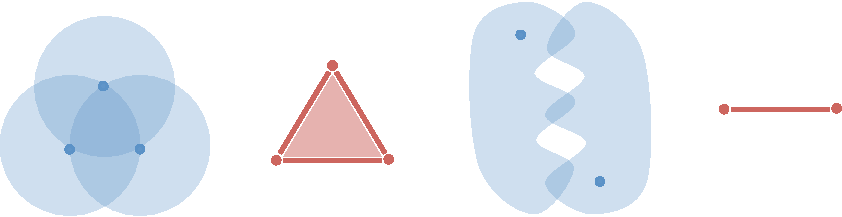
\includegraphics[width=\textwidth]{nerves.pdf}
\caption{Covers and Their Nerves}
\label{fig:nerves}
\end{figure}

In Figure~\ref{fig:nerves} we have drawn two different arrangements of open sets and their corresponding nerves, which we have represented graphically to the right. We have added points to each open set to make it clear how many open sets are in the cover. Note that in general, there is nothing to prevent a disconnected open set from being marked by a single label. 

The nerve is purely an algebraic and combinatorial model for the cover --- it need not respect the topology of the union. However, the \textbf{nerve theorem}\index{nerve theorem} of Leray and Borsuk~\cite{leray45,borsuk-nerve} states that if the intersections are contractible then the nerve and the union have the same homotopy type. The example on the left in Figure~\ref{fig:nerves} gives a positive example of the nerve lemma, whereas the example on the right gives a negative one.

The definition of a sheaf or cosheaf requires the synthesis of covers and data. We now introduce the functor that assigns data to open sets.
\begin{defn}[Pre-Sheaf and Pre-Cosheaf]\index{presheaf}\index{pre-cosheaf}
	A \textbf{pre-sheaf} is a functor $F:\Open(X)^{op}\to\dat$ and a \textbf{pre-cosheaf} is a functor $\hF:\Open(X)\to\dat$. If $V\subset U$, then we usually write the \textbf{restriction map} as $\rho_{V,U}^F:F(U)\to F(V)$ and the \textbf{extension map} as $r^{\hF}_{U,V}:\hF(V)\to\hF(U)$. Often we omit the superscript $F$ or $\hF$.
\end{defn}

If one imagines the pre-cosheaf that associates a copy of the field $k$ to every connected component of an open set, then the following diagrams of vector spaces emerge from Figure~\ref{fig:nerves}:
\[
\xymatrix@R=1em{ & k & \\ k \ar[ru] \ar[dd] & & k \ar[lu] \ar[dd]\\ & \ar[lu] \ar[uu] \ar[ru] k \ar[dl] \ar[dd] \ar[dr] & \\ k & & k \\ & \ar[lu] \ar[ru] k &}
\qquad \qquad \qquad
\xymatrix@R=1em{ & & \\ & & \\ k & k^3 \ar[l] \ar[r] & k \\ & & \\ & &}
\]
We will examine various ways for computing the colimits of these diagrams explicitly. Since the colimits occur over simplicial complexes, we introduce a structure theorem that allows us to use coequalizers. In the vector space case, this reduces to linear algebra --- the colimit will be $H_0$ of a suitable chain complex.

We want to express the fact that since the colimit of a cover $N(\covU)\to \Open(X)$ is just the union $U=\cup U_i$, the data associated to $U$ should be expressible as the colimit of data assigned to the nerve. Moreover, this should be independent of which cover we take. Examples where this does not occur are given in Example~\ref{ex:nonlocalpresheaf} and Example~\ref{ex:inconsistentpresheaf}.
\begin{defn}[Sheaves and Cosheaves]\label{defn:sheaf}\index{sheaf!definition of}\index{cosheaf!definition of}
	Suppose $F$ is a pre-sheaf and $\hF$ is a pre-cosheaf, both of which are valued in $\dat$. Suppose $\covU=\{U_i\}$ is an open cover of $U$. We say that $F$ is a \textbf{sheaf on $\covU$} if the unique map from $F(U)$ to the limit of $F\circ \iota^{op}_{\covU}$, written 
	\[
	F(U)\to \varprojlim_{I\in N(\covU)} F(U_I)=:F[\covU],
	\]
	is an isomorphism. Similarly, we say $\hF$ is a \textbf{cosheaf on $\covU$} if the unique map from the colimit of $\hF\circ\iota_{\covU}$ to $\hF(U)$, written
	\[
	\hF[\covU]:=\varinjlim_{I\in N(\covU)} \hF(U_I) \to \hF(U),
	\]
	is an isomorphism. We say that $F$ is a \textbf{sheaf} or $\hF$ is a \textbf{cosheaf} if for every open set $U$ and every open cover $\covU$ of $U$, $F(U)\to F[\covU]$ or $\hF[\covU]\to \hF(U)$ is an isomorphism. For a catchy slogan, we say 
\begin{quote}
	\begin{center}
	\emph{On an open set (co)sheaves turn different covers into isomorphic (co)limits}.
\end{center}
\end{quote}
\end{defn}
\begin{rmk}[Stable Under Finite Intersection]
	Most authors do not introduce the nerve as any part of the definition of a sheaf or cosheaf. Instead, some will require that the cover $\covU$ is ``stable under finite intersection,'' i.e. if $U_i,U_j\in\covU$, then $U_i\cap U_j\in\covU$. This allows those authors to just consider the limit or colimit over the cover and not over some auxiliary construction, like we have done. This works because one can take any cover and then add the intersections after the fact, but this tends to be done unconsciously and without any warning to the reader. Our approach is equivalent to that approach, but we believe it has some added benefits.
\end{rmk}

We have not stated any requirements on the data category $\dat$, but in order to even parse the statement of the (co)sheaf axiom we require that the (co)limits coming from such covers exist. For the most part, we will work in categories where all limits and colimits exist. In analogy with analysis, a category where the limit of any diagram $F:I\to\dat$ exists is called \textbf{complete}. Similarly, if the colimit of an arbitrary diagram exists, we say $\dat$ is \textbf{co-complete}. The category $\Vect$ is both complete and co-complete.
	
A particular consequence of the axiom is that for a sheaf, $F(\emptyset)$ must be the limit over covers of the empty set, but since there are no such covers\footnote{Alternatively one argues that the empty set covers itself and hence the value there is chosen to be the initial/terminal object of the category $\dat$.} this is the limit over the empty diagram, i.e. $\Cone(\emptyset)=\dat$, whose terminal object is the terminal object of $\dat$. Similarly, for a cosheaf $\hF(\emptyset)$ must be the initial object in $\dat$. For $\dat=\Vect$ the initial and terminal objects coincide with the zero vector space.
	
It is true that if $\dat$ has pullbacks (see Example~\ref{ex:pullback} in Section~\ref{sec:categories}) and a terminal object then it has all finite limits. The dual statement that having an initial object and pushouts (see Example~\ref{ex:pushout}) implies finitely co-complete is also true. Thus, if one focuses on sheaves and cosheaves valued in $\vect$ (the category of finite dimensional vector spaces and linear maps), then the collection of covers of $U$ one can consider must be restricted. In particular, if the sheaf or cosheaf axiom holds for open covers with two sets, then we can only guarantee that it holds for covers with finitely many open sets. As a purely philosophical point, one wonders whether working with the cover of the complement of the Cantor set given by
\[
	\covU=\{(\frac{3k+1}{3^n},\frac{3k+2}{3^n})\subset[0,1] | 0\leq k\leq 3^{n-1}-1, \, 0\leq n<\infty\}
\]
would ever be computationally tractable. One might wish to systematically revise the notion of a ``cover,'' and this would lead to the notion of a \textbf{Grothendieck site}, which we do not address here.

We now examine the axioms just for covers with only two open sets.

\begin{figure}[ht]
\centering
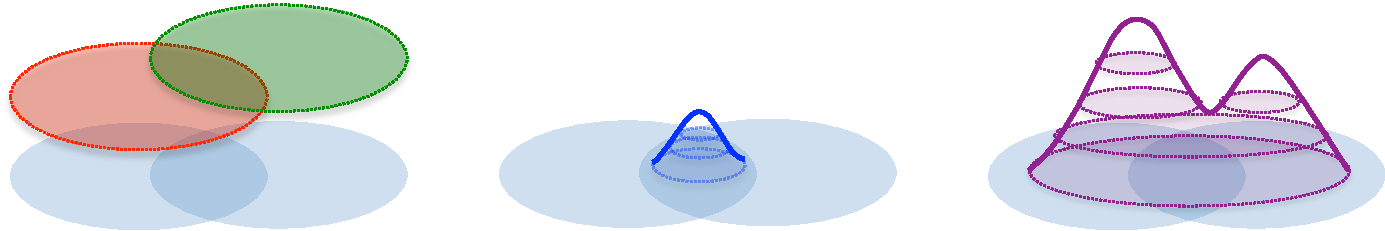
\includegraphics[width=\textwidth]{fun_sheaves.pdf}
\caption{Sheaves and Cosheaves of Functions}
\label{fig:fun_sheaves}
\end{figure}

\begin{ex}[Cover by Two Sets]\index{sheaf!axiom for two opens}\index{cosheaf!axiom for two opens}\index{cosheaf!of compactly supported functions}
Suppose $\dat=\Set$, and suppose $\covU=\{U_1,U_2\}$ is a cover of $U$. The sheaf condition says that
\[
	F(U)\cong\{(s_1,s_2)\in F(U_1)\prod F(U_2) | \rho_{U_{12},U_1}(s_1)=\rho_{U_{12},U_2}(s_2)\}=:F[\covU],
\]
i.e. $F(U)$ lists the set of consistent choices of elements from $F(U_1)$ and $F(U_2)$. In particular, $F[\covU]$ is a sub-object of the product of $F(U_1)$ and $F(U_2)$. For an example, one can let $F$ be the assignment
\[
	U \rightsquigarrow \{f:U\to\RR \,|\, \mathrm{continuous} \}.
\]
The sheaf axiom then says in order for two functions (or sections) $s_1=f_1:U_1\to\RR$ and $s_2=f_2:U_2\to\RR$ to determine an element in $U=U_1\cup U_2$ it is necessary and sufficient that the functions $f_1(x)$ and $f_2(x)$ agree on the overlap $U_{12}=U_1\cap U_2$.

The cosheaf condition for $\dat=\Set$ is slightly strange. It says that
\[
	\hF(U)\cong (\hF(U_1)\coprod \hF(U_2))/\sim
\]
\[
	s_1\sim s_2 \, \Leftrightarrow \, \exists s_{12} \quad s_1=r_{U_1,U_{12}}(s_{12}) \quad  s_2=r_{U_2,U_{12}}(s_{12}).
\]
	In contrast to the sheaf case, the notion of consistent choices no longer applies for cosheaves, because it requires thinking in terms of quotient objects --- something human beings are not accustomed to. However, a useful analogy is that one must subtract out or identify those elements that might be counted twice because they come from the intersection. For an example similar in spirit to the sheaf of real-valued functions, we begin by considering the pre-cosheaf of compactly supported functions gotten by the assignment
	\[
		U \rightsquigarrow \{f:U\to\RR \,|\, \mathrm{continuous}\,\,\mathrm{and}\,\,\mathrm{compactly}\,\,\mathrm{supported} \}.
	\]
	Extending by zero provides the extension map and identifying the two copies of a function whose support is contained in $U_{12}=U_1\cap U_2$ prevents double counting on $U$. However, this is not all that the cosheaf axiom requires. Any compactly supported function should appear as one supported in $U_1$ or $U_2$, but this is not always true. Some compactly supported functions are not compact when restricted to any particular open set in a cover. Thus, this pre-cosheaf is \emph{not} a cosheaf.
	
	The reader familiar with partitions of unity will realize that if $X$ a paracompact Hausdorff space then we can express any compactly supported function $f(x)$ defined on all of $U$ as a \emph{sum} of compactly supported functions on $U_1$ and $U_2$. By taking a partition of unity subordinate to the cover $\covU$ we get two functions $\lambda_1(x)$ and $\lambda_2(x)$ such that
	\[
		f(x)=f_1(x)+f_2(x) \quad \mathrm{where} \quad f_1(x):=\lambda_1(x)f(x) \quad \mathrm{and} \quad f_2(x):=\lambda_2(x)f(x).
	\]
	By carrying out the colimit in a data category equipped with sums, such as $\dat=\Vect$ of $\Ab$, then compactly supported functions do define a cosheaf valued there.

	More generally, if $\dat=\Vect$, then the cosheaf axiom for the cover says the sequence
	\[
	\hF(U_{12}) \to \hF(U_1)\oplus\hF(U_2) \to \hF(U) \to 0
	\]
	is exact, where the maps are $(-r_{U_1,U_{12}},r_{U_2,U_{12}})$ and $r_{U,U_2}+r_{U,U_1}$. Dually, the sheaf axiom says the dual sequence
	\[
	0 \to F(U)\to F(U_1)\times F(U_2) \to F(U_{12})
	\]
	is exact, where the second map is $\rho_{U_{12},U_2}+\rho_{U_{12},U_1}$ and the first map is $(-\rho_{U_1,U},\rho_{U_2,U})$.
\end{ex}

\section{Limits and Colimits over Covers: a Structure Theorem}
\label{subsec:cover_structure}\index{limit!over a cover}\index{colimit!over a cover}

The sheaf and cosheaf axioms as stated are meant to emphasize that if one is comfortable with the operations of limits and colimits, then one is already comfortable with sheaves and cosheaves. However, the limits and colimits considered in Definition~\ref{defn:sheaf} have a special structure. This structure comes from the fact that the indexing category --- the nerve --- is a simplicial complex.

The first observation one can make is that for any functor $F:N(\covU)^{op}\to\dat$ the limit can be thought of as ``sitting inside'' the product over the vertices --- the vertices corresponding to the elements of the cover through the nerve construction. Dually, the colimit of a functor $\hF:N(\covU)\to\dat$ can be thought of as a quotient of the coproduct of the functor over the vertices. Said using formulas, this is
\begin{equation*}
	\varprojlim F \hookrightarrow \prod F(i) \qquad \coprod \hF(i) \twoheadrightarrow \varinjlim \hF.
\end{equation*}
The way to see this is to note that any cone or cocone's morphism must factor through a vertex. However, the difference between the limit or colimit from the functor's aggregate value on vertices is measured by edges in the nerve. This is a reflection of a more general theorem, which we now state.

\begin{thm}\label{thm:limits_equal}\index{limit!as an equalizer}\index{colimit!as a coequalizer}
	A category $\dat$ has all (co)limits of an appropriate size if it has all (co)products and (co)equalizers of same such size. Here ``size'' corresponds to the cardinality of the indexing category of the (co)limit in question.
\end{thm}
\begin{proof}[Proof (Sketch)]
One should consult~\cite[Prop. 5.22-3]{awodey} for a complete proof. To give the reader the idea, one can compute the limit of $F:I\to\dat$ by taking the product over all the objects $x\in I$ and separately the product over all morphisms in the indexing category $I$. The limit is isomorphic to the equalizer going from the first product to the latter, i.e.
\begin{equation*}
 \xymatrix{ \varprojlim F \ar[r] & \prod_{x\in I} F(x) \ar@<-.5ex>[r] \ar@<.5ex>[r] & \prod_{x\to x'} F(x')}.
\end{equation*}
By dualizing, one can prove the analogous result for colimits. 
\end{proof}

This theorem gives us effective means for computing limits and colimits for general data types. We now specialize this result to the limits and colimits pertinent to sheaves and cosheaves.

\subsection{Rephrased as Equalizers or Co-equalizers}
\label{subsubsec:equalizers}
\index{sheaf!axiom as an equalizer}\index{cosheaf!axiom as a coequalizer}

The method outlined in Theorem~\ref{thm:limits_equal} for computing limits and colimits contains too much redundant information for the case $I=N(\covU)^{op}$. As such, we state the precise, simplified formulation here. The sheaf and cosheaf axioms can be rephrased as saying that the following sequences
\begin{equation*}
	\xymatrix{F(U) \ar[r]^-e & \prod F(U_i) \ar@<-.5ex>[r]_-{f^+} \ar@<.5ex>[r]^-{f^-} & \prod_{i<j} F(U_i\cap U_j)}
\end{equation*} 
\begin{equation*}
\xymatrix{\coprod_{i<j}\hF(U_i\cap U_j) \ar@<-.5ex>[r]_-{g^-} \ar@<.5ex>[r]^-{g^+} & \coprod \hF(U_i) \ar[r]^-u & \hF(U)}
\end{equation*}
are an equalizer and a co-equalizer respectively. 

\begin{exr}
Prove that the limit or colimit over the nerve of a cover can be determined after considering only the elements of the cover and their pairwise intersections. Do this by observing that the limit or colimit over the 1-skeleton\footnote{In higher homotopy analogs of sheaves and cosheaves one works over the whole \v{C}ech tower of a cover~\cite{dugger-hypercovers,douglas2007sheaves,gwilliam-stacks}.} of the nerve defines a cone or cocone over the whole nerve and employing universal properties. Then apply the equation from Theorem~\ref{thm:limits_equal} and its dual version to prove that the re-written axioms of Section~\ref{subsubsec:equalizers} and Section~\ref{subsubsec:exactness} are correct.
\end{exr}

To describe the maps explicitly requires some work. First, we choose an ordering of the indexing set of the cover $\covU=\{U_i\}_{i\in\Lambda}$. To specify a map to a product it suffices to specify maps to each factor of the product. Similarly, maps from a coproduct are specified by maps from each factor. This is summarized by the identities 
	\[
	\Hom(X,\prod_i Y_i)\cong \prod_i\Hom(X,Y_i) \qquad \mathrm{and} \qquad \Hom(\coprod_i X_i,Y)\cong\prod_i \Hom_i(X_i,Y).
	\]
To define the maps $e$ and $u$ we declare $e_i:=\rho_{U_i,U}$ and $u_i:=r_{U,U_i}$. For the maps $f^{\pm}$ and $g^{\pm}$ we define for each pair $i<j$ the maps
	\[
	f^+_{ij}:=\rho_{ij,j}\circ\pi_j \quad f^-_{ij}:=\rho_{ij,i}\circ\pi_i \qquad g^+_{ij}:=r_{j,ij}\circ\iota_{ij} \quad g^-_{ij}:=r_{i,ij}\circ\iota_{ij}
	\]
where $\pi_i:\prod F(U_i)\to F(U_i)$ is the natural projection and $\iota_{ij}:\hF(U_{ij})\to \coprod \hF(U_{ij})$ is the natural inclusion.
	
The reader might find it helpful to think of the maps in between the products as being represented by matrices. In the case of a cover with three elements $\covU=\{U_1,U_2,U_3\}$ all of whose pairwise intersections are non-empty, we can write
	\[
	f^+=\begin{bmatrix} \ast & \rho_{12,2} & \ast  \\  \ast & \ast & \rho_{13,3} \\ \ast & \ast & \rho_{23,3}\end{bmatrix} \quad f^-=\begin{bmatrix} \rho_{12,1} &\ast  &\ast  \\ \rho_{13,1} & \ast  & \ast \\ \ast & \rho_{23,2} &\ast \end{bmatrix}.
	\]
	The equalizer condition now reads that $f^+(s_1,s_2,s_3)=f^-(s_1,s_2,s_3)$, i.e. 
	\[
	(\rho_{12,2}(s_2),\rho_{13,3}(s_3),\rho_{23,3}(s_3))=(\rho_{12,1}(s_1),\rho_{13,1}(s_1),\rho_{23,2}(s_2)).
	\]
	
\subsection{Rephrased as Exactness}\label{subsubsec:exactness}
\index{sheaf!axiom as an exact sequence}\index{cosheaf!axiom as an exact sequence}

If $\dat=\Vect$, then we can add and subtract maps and look for kernels and cokernels instead of equalizers and co-equalizers. The sheaf and cosheaf axioms then reduce to linear algebra. The modified axioms now read as
\[
	\xymatrix{0 \ar[r] & F(U) \ar[r] & \prod F(U_i) \ar[r]^-{d^0} & \prod_{i<j} F(U_i\cap U_j)}
\]
\[
	 \xymatrix{\bigoplus_{i<j}\hF(U_i\cap U_j) \ar[r]^-{\partial_1} & \bigoplus \hF(U_i) \ar[r] & \hF(U) \ar[r] & 0}
\]
where $d^0$ is the matrix whose rows are parametrized by pairs $i<j$ and whose columns are parametrized by $k$ with entries given by $d^0_{ij,k}=[k:ij]\rho_{ij,k}$ where 
	\[
		[k:ij]=\left\{\begin{array}{ll} 0 & \mathrm{if} \,\, k\neq i\neq j \\
		1 & \mathrm{if} \,\, k=j\\
		-1 & \mathrm{if} \,\, k=i\end{array}\right.
	\]
The matrix $\partial_1$ is similarly defined except that the rows are indexed by $k$ and columns are indexed by pairs $i<j$ with entries $(\partial_1)_{k,ij}=[k:ij]r_{k,ij}$. Thus the sheaf axiom says that $F(U)\cong \ker(d^0)$ and the cosheaf axiom says that $\hF(U)\cong \coker (\partial_1)$.
	
In our example of a three set cover $\covU=\{U_1,U_2,U_3\}$ all of whose pairwise intersections are non-empty, the definition of $d^0$ corresponds to taking $f^+ - f^-$, i.e.
	\[
		d^0=f^+ - f^- =\begin{bmatrix} -\rho_{12,1} & \rho_{12,2} & 0 \\ -\rho_{13,1} & 0 & \rho_{13,3} \\ 0 & -\rho_{23,2} & \rho_{23,3}\end{bmatrix}
	\]
where each of the $\rho_{ij,k}$'s need to be filled in with some matrix representative of that linear map. The kernel is then identified with $F[\covU]$.

\section{\v{C}ech Homology and Cosheaves}\label{subsec:cech}
\index{Cech@\v{C}ech homology}

In Section~\ref{subsubsec:equalizers} we rephrased the limits and colimits coming from covers as equalizers and coequalizers. For the data category $\dat=\Vect$ we showed how to reinterpret this as an exact sequence. This perspective is indicative of a deeper and more computational idea, namely that of homology. We now show how to associate to any pre-cosheaf\footnote{Or pre-sheaf, but we'll leave it to the reader to dualize.} of vector spaces $\hF$ and an open cover $\covU=\{U_i\}_{i\in\Lambda}$ a complex of vector spaces whose zeroth homology computes $\hF[\covU]$. This allows us to compute the homology of data.

\begin{defn}[\v{C}ech Homology]
	Given a pre-cosheaf of vector spaces $\hF$ and an open cover $\covU=\{U_i\}_{i\in\Lambda}$, we define the \textbf{\v{C}ech homology on $\covU$} to be the homology of the complex
\[
	(\check{C}_{\bullet}(\covU;\hF),\partial_{\bullet}) \qquad \mathrm{where} \qquad \check{C}_p(\covU;\hF):=\bigoplus_{|I|=p+1} \hF(U_I) \qquad \mathrm{for} \qquad I\in N(\covU).
\]
By choosing an ordering on the index set $\Lambda$, we define the differential by extending the formula defined on elements $s_I\in\hF(U_I)$ by linearity, i.e.
\[
	\partial_p:C_p(\covU;\hF)\to C_{p-1}(\covU;\hF) \qquad \partial_p(s_I):=\sum_{k=0}^p (-1)^k r_{U^{(k)}_I,U_I}(s_I),
\]
where the symbol $U^{(k)}_I=U_{i_0}\cap \ldots \cap U_{i_{k-1}}\cap U_{i_{k+1}} \cap \ldots  U_{i_p}$ indicates the intersection that omits the $k$th open set.
Thus we can define by the usual formula the $p$th \textbf{\v{C}ech homology group}
\[
	\check{H}_p(\covU;\hF):=\frac{\ker \partial_p}{\im \partial_{p+1}} \qquad \mathrm{i.e.} \qquad H_p(\check{C}_{\bullet}(\covU;\hF)).
\]
\end{defn}

To guarantee that \v{C}ech homology is well-defined we verify the following lemma:
\begin{lem}\index{Cech@\v{C}ech homology!$\partial^2=0$}
	The differential $\partial$ in the \v{C}ech complex for a cover $\covU$ and a pre-cosheaf $\hF$ of vector spaces satisfies $\partial_{p}\circ\partial_{p+1}=0$.
\end{lem}
\begin{proof}
The combinatorial nature of the nerve of a cover guarantees that $\partial^2=0$. Specifically, there are two ways of going between incident simplices of dimension differing by two. Thus, we get the following diagram of open sets and data:
\[
	\xymatrix{ & U^{(j,k)}_I & \\
	U^{(j)}_I \ar[ur] & & U^{(k)}_I \ar[ul] \\
	& U_I \ar[ul] \ar[ur] \ar[uu] &}
	\qquad \qquad
	\xymatrix{ & \hF(U^{(j,k)}_I) & \\
	\hF(U^{(j)}_I) \ar[ur] & & \hF(U^{(k)}_I) \ar[ul] \\
	& \hF(U_I) \ar[ul] \ar[ur] \ar[uu] &}
\]

Let's follow a typical element $s_I\in\hF(U_I)$ through the diagram on the right upon applying the formula $\partial\circ\partial$. First note that the fact that $\hF$ is a pre-cosheaf implies that the square commutes, i.e. 
\[
r_{U^{(j,k)}_I,U^{(j)}_I}\circ r_{U^{(j)}_I,U_I}(s_I)=r_{U^{(j,k)}_I,U^{(k)}_I}\circ r_{U^{(k)}_I,U_I}(s_I)=r_{U^{(j,k)}_I,U_I}(s_I).
\] 
The first application of $\partial$ yields $(-1)^j r_{U^{(j)}_I,U_I}(s_I)$ and $(-1)^k r_{U^{(k)}_I,U_I}(s_I)$ as just two components in the formula for $\partial(s_I)$. Assuming $j<k$ and applying the definition of the boundary map to elements in $\hF(U^{(j)}_I)$ implies that we must actually delete the $k-1$st entry of $I-\{j\}$ since removing $j$ has caused everything above $j$ to shift down in the ordered list. Thus the image of $\partial^2(s_I)$ in $\hF(U^{(j,k)}_I)$ is
\[
	(-1)^{k-1}(-1)^jr_{U^{(j,k)}_I,U_I}(s_I) + (-1)^{k}(-1)^jr_{U^{(j,k)}_I,U_I}(s_I)=0.
\]
\end{proof}

\begin{ex}\index{Cech@\v{C}ech homology!example of}
	Consider the covers in Figure~\ref{fig:nerves}. The pre-cosheaf we described there assigned to each connected component of an open set a copy of the field $k$. First we consider the cover on the left of Figure~\ref{fig:nerves} with three open sets. We label the three vertices of the nerve, starting with the bottom left one and working counter-clockwise, $x,y$ and $z$ respectively. The \v{C}ech complex takes the form
	\[
		\xymatrix{k_{xyz} \ar[r]^-{\partial_2} & k_{xy}\oplus k_{xz}\oplus k_{yz} \ar[r]^{\partial_1} & k_x\oplus k_y \oplus k_z \ar[r] & 0 }
	\]
	where, using the lexicographic ordering for a basis, the matrix representatives for $\partial_2$ and $\partial_1$ take the following form:
	\[
		\partial_2=\begin{bmatrix} 1 \\ -1 \\ 1\end{bmatrix} \qquad \qquad  \partial_1=\begin{bmatrix} -1 & -1 & 0 \\ 1 & 0 & -1 \\ 0 & 1 & 1\end{bmatrix}
	\]
	One can easily verify that the $\ker \partial_1=\im \partial_2$ and consequently $\check{H}_1=0$. Furthermore, $\check{H}_0\cong k$, which happens to reflect that the union has one connected component.
	Similarly, one can consider the cover at the right of Figure~\ref{fig:nerves}. The \v{C}ech complex for this cover and the same pre-cosheaf is as follows:
	\[
		\xymatrix{k^3 \ar[r]^{\partial_1} & k^2 \ar[r] & 0 } \qquad \mathrm{where} \qquad \partial_1=\begin{bmatrix} -1 & -1 & -1 \\ 1& 1 & 1\end{bmatrix}
	\]
	Clearly $\check{H}_0\cong k$, whose dimension agrees with the number of connected components of the union, but also $\check{H}_1\cong k^2$, which witnesses the presence of two holes in the union.
\end{ex}

One can dually define \v{C}ech cohomology with coefficients valued in a pre-sheaf $F$. The discussion of Section~\ref{subsubsec:exactness}, along with the examples just presented, can be interpreted as saying a pre-sheaf $F$ or pre-cosheaf $\hF$ is a sheaf or cosheaf if and only if
	\[
	F(U)\cong \check{H}^0(\covU;F) \qquad \mathrm{or} \qquad \check{H}_0(\covU;\hF)\cong \hF(U).
	\]
for any choice of cover $\covU$ of $U$.
	
We would like to use this isomorphism to supply examples of sheaves and cosheaves from standard machinery in algebraic topology. Suppose one has an independent notion of homology, such as singular homology, and one can show it is isomorphic to \v{C}ech homology for suitably fine covers (see Section~\ref{subsec:refinement} to see why fineness matters) on nice spaces, then one can also define a cosheaf using those values. To make this rigorous, and to also provide a useful criterion for proving when a pre-cosheaf is a cosheaf, we recall a theorem:

\begin{thm}\label{thm:MV_cosheaf}\index{cosheaf!Mayer-Vietoris}\index{Mayer-Vietoris}
	Suppose $\hF$ is a pre-cosheaf, then $\hF$ is a cosheaf if and only if the following the following two properties hold
	\begin{itemize}
		\item For all open sets $U$ and $V$ the following sequence is exact
		\[
			\hF(U\cap V) \to \hF(U)\oplus \hF(V) \to \hF(U\cup V) \to 0.
		\]
		The first morphism is $(-r_{U,U\cap V},r_{V,U\cap V})$ and the second is $r_{U\cup V,U}+r_{U\cup V,V}$.
		\item If  $\{U_{\alpha}\}$ is directed upwards by inclusion, i.e. for for every pair $U_{\alpha}$ and $U_{\beta}$ there exists $U_{\gamma}$ containing both, then the canonical map
		\[
			\varinjlim_{\alpha} \hF(U_{\alpha}) \to \hF(\cup U_{\alpha})
		\]
		is an isomorphism. 
	\end{itemize}
	Dually, turning arrows around and using inverse limits gives a useful criterion for determining when a pre-sheaf is a sheaf.
\end{thm}
\begin{proof}
	Using induction one can prove that the cosheaf property for two sets implies the cosheaf property for finitely many sets (see~\cite[p. 418]{Bredon} for a proof). We now show that this implies the cosheaf axiom for arbitrary covers. Suppose $\{U_{\alpha}\}_{\alpha\in\Lambda}$ is a cover indexed by a potentially large, but ordered set $\Lambda$. For each finite subset $I\subset \Lambda$ we know that
	\[
	\bigoplus_{\alpha<\beta\in I} \hF(U_{\alpha,\beta}) \to \bigoplus_{\alpha\in I} \hF(U_{\alpha}) \to \hF(\bigcup_{\alpha\in I} U_{\alpha}) \to 0
	\]
	is exact. We know that the collection of finite subsets $I$ forms a directed system and that in $\Vect$ direct limits preserve exactness. As such we have that
	\[
	\varinjlim_I \bigoplus_{\alpha<\beta\in I} \hF(U_{\alpha,\beta}) \to \varinjlim_I \bigoplus_{\alpha\in I} \hF(U_{\alpha}) \to \varinjlim_I \hF(\bigcup_{\alpha\in I} U_{\alpha}) \to 0
	\]
	is exact as well, but by using the second property and the fact that the direct limit of the $I$'s is $\Lambda$ we have
	\[
		\bigoplus_{\alpha<\beta\in \Lambda} \hF(U_{\alpha,\beta}) \to \bigoplus_{\alpha\in \Lambda} \hF(U_{\alpha}) \to \hF(\bigcup_{\alpha\in \Lambda} U_{\alpha}) \to 0
	\]
	is exact. This proves the reverse direction. The other direction is clear.
\end{proof}

This theorem then provides us with a useful example of a cosheaf that we have implicitly used to generate examples. We now make this example explicit.

\begin{ex}\index{cosheaf!given by $H_0$}
	The assignment to an open set $U$ the $0$th singular homology of $U$
	\[
		U \rightsquigarrow H_0(U;k)
	\]
	is a cosheaf. This follows from the fact that the singular chain complex (see later for a definition) $C_{\bullet}(-;k)$ can be defined for any subset $U$ of $X$ and homology commutes with direct limits, thus the second property of the theorem holds. The first property in the theorem follows from exactness at the last two spots in the Mayer-Vietoris sequence:
	\[
	\xymatrix{
		            & H_1(U\cap V;k)\ar@{->}[r] & H_1(U;k)\oplus H_1(V;k) \ar@{->}[r]
		                   & H_1(U\cup V;k)  \ar `r[d] `_l[lll] ^{} `^d[dlll] `^r[dll] [dll] \\
		             & H_{0}(U\cap V;F)\ar@{->}[r] & H_0(U;k) \oplus H_0(V;k) \ar@{->}[r]
		                   & H_0(U\cup V;k) \ar[r] & 0 \\
		}
	\]
\end{ex}

The moral from this example is that, in essence,
\begin{quote}
	\begin{center}
	\emph{Any functor that satisfies Mayer-Vietoris is a cosheaf.}
\end{center}
\end{quote}

\section{Refinement of Covers}\label{subsec:refinement}
\index{cover!refinement of}

We have defined the sheaf and cosheaf axioms for a cover $\covU$. The coarsest possible cover of an open set $U$ is the cover with one element $\{U\}$. Thus, one way of interpreting the sheaf and cosheaf axiom is that $F[\covU]$ and $\hF[\covU]$ are independent of the cover chosen. A logical question to ask is if the axiom holds for some cover, but not all, then for what other covers does the axiom hold? To answer this question, we review some relevant concepts.

\begin{defn}[Refinement of Covers]
	Suppose $\covU$ and $\covU'$ are covers of $U$, then we say that $\covU'$ \textbf{refines} $\covU$ if for every $U_i'\in\covU'$ there is a $U_j\in\covU$ and an inclusion $U_i'\to U_j$. Note that every cover refines the trivial cover $\{U\}$.
\end{defn}

\begin{defn}\index{category!of covers}
The refinement relation endows the collection of covers of $U$ with the structure of a category $\Cov(U)$, whose objects are covers $\covU$ with a unique morphism $\covU'\to\covU$ if the former refines the latter.
\end{defn}

Note that if $U_{i_1}'\to U_{j_1}$ and $U'_{i_2}\to U_{j_2}$, then $U'_{i_1}\cap U_{i_2}'\to U_{j_1}\cap U_{j_2}$. So a refinement induces a functor between nerves, but it depends on which inclusions were chosen.
\[
\xymatrix{ & \Open(X) & \\ N(\covU') \ar[ru] \ar[rr] & & N(\covU) \ar[lu]} \qquad \xymatrix{ & \Open(X)^{op} & \\ N(\covU')^{op} \ar[ru] & & N(\covU)^{op} \ar[lu] \ar[ll]}
\]

The next lemma shows that these choices don't matter on the level of limits and colimits for pre-sheaves and pre-cosheaves.

\begin{lem}\index{presheaf!behavior under refinement}\index{pre-cosheaf!behavior under refinement}
	Let $\hF$ and $F$ be a pre-cosheaf and a pre-sheaf respectively. Suppose $\covU'$ refines another cover $\covU$ of an open set $U$. Then there are well-defined maps
	\[
	\hF[\covU']\to \hF[\covU] \qquad \mathrm{and} \qquad F[\covU]\to F[\covU'],
	\]
	i.e. we get functors $\hF:\Cov(U)\to\dat$ and $F:\Cov(U)^{op}\to\dat$.
\end{lem}
\begin{proof}
We'll detail the proof for a pre-cosheaf $\hF$ since the case for pre-sheaves can be found in the literature or obtained here via dualizing appropriately. A refinement $\covU'\to\covU$ defines a natural transformation $\hF\circ \iota_{\covU'}\Rightarrow \hF\circ \iota_{\covU}$. The colimit defines a natural transformation from $\hF\circ \iota_{\covU}$ to the constant diagram $\hF[\covU]$. Since the composition of natural transformations is a natural transformation, this induces a cocone $\hF\circ\iota_{\covU'}\Rightarrow \hF[\covU]$ which, by the universal property of the colimit, defines a unique induced map there, i.e.
\[
\hF\circ \iota_{\covU'}\Rightarrow \hF\circ \iota_{\covU}\Rightarrow \hF[\covU] \quad \mathrm{implies} \quad \exists!\, \hF[\covU']\to\hF[\covU].
\]
However, if in choosing the inclusions for the refinement we had made a different set of choices, $U_i'\to U_k$ rather than $U_j$, then a priori we might have expected different maps $\hF[\covU']\to\hF[\covU]$. Let us show this choice does not matter. If there is a choice, then we can take $U'_i\to U_j\cap U_k$ as a common refinement. As a consequence of $\hF$ being a functor from the open set category, the different maps to the colimit must agree, as they factor through whatever is assigned on the intersection, i.e. the following diagram commutes:
\[
\xymatrix{& & \hF(U_j) \ar[d] \\
\hF(U_i')  \ar[r] \ar[rru] \ar[rrd]& \hF(U_j\cap U_k) \ar[ru] \ar[rd] \ar[r] & \hF[\covU] \\
& & \hF(U_k) \ar[u]} 
\]
\end{proof}

\begin{cor}\label{cor:refined_axiom}\index{sheaf!behavior under refinement}\index{cosheaf!behavior under refinement}
	If $\hF$ is a cosheaf or $F$ is a sheaf for the cover $\covU'$, then it is a cosheaf or sheaf for every cover it refines.
\end{cor}
\begin{proof}
	Suppose we have a series of refinements
	\[
	\covU'\to\covU\to \{U\}.
	\] 
	To say that $\hF$ or $F$ is cosheaf or sheaf for $\covU'$ is to say that the following induced maps are isomorphisms:
	\[
	\xymatrix{\hF[\covU'] \ar[r] \ar@/^2pc/[rr]^{\cong} & \hF[\covU] \ar[r] & \hF(U)} \qquad \xymatrix{F(U) \ar[r] \ar@/^2pc/[rr]^{\cong} & \hF[\covU] \ar[r] & \hF[\covU']}
	\]
	However, by functoriality, the factored maps must themselves be isomorphisms, i.e.
	\[
	\xymatrix{\hF[\covU]\ar[r]^{\cong} & \hF(U)} \qquad \xymatrix{F(U) \ar[r]^{\cong} & F[\covU]}.
	\]
\end{proof}
We will make use of this corollary as we begin to consider sheaves and cosheaves on spaces where there is a finest cover. Checking the sheaf or cosheaf axiom there then guarantees it for all covers.

\section{Generalities on Sheaves and Cosheaves}
\label{subsec:generalities}

Sheaves have proved to be highly successful tools in pure mathematics over the past 60-70 years. This is largely because sheaves provide precise mechanisms for determining global unknowns from local knowns. These mechanisms are greatly enhanced by considering the operations such as $\Hom$ and $\otimes$ on sheaves, as well as the pushforward and pullback of a sheaf along a map, which we define in Section~\ref{subsec:six_ops}. Some of these operations are only available after applying a certain repair to turn a presheaf into a sheaf, also known as \textbf{sheafification}, which we define in Section~\ref{subsec:sheafification} after some preliminary discussion of examples.

One would like to know if a similar story is true for cosheaves. After all, any functor $\hF:\Open(X)\to\dat$ is exactly equivalent to specifying a functor $F:\Open(X)^{op}\to\dat^{op}$. However, certain asymmetries prevent such an observation from being as useful as one might hope. These asymmetries are outlined in Section~\ref{subsec:failure_to_commute} and obstruct the use of Grothendieck's version of sheafification to define an analogous \textbf{cosheafification}. However, we prove that such a device must exist in Section~\ref{subsec:cosheafification} without knowing a particular construction.

\subsection{Pre-sheaves and their Associated Sheaves}\label{subsec:sheafification}

Sheaves are fundamentally local structures. Informally stated, a pre-sheaf can fail to be a sheaf in two independent ways:
\begin{itemize}
\item \emph{Non-Local}: If a pre-sheaf has a section $s\in F(U)$ that cannot be constructed from sections over smaller open sets in $U$ --- a cover of $U$, for example --- then $F$ fails to be a sheaf.
\item \emph{Inconsistent}: If a pre-sheaf has a pair of sections $s\neq t\in F(U)$ such that when restricted to every smaller open set they define the same section, then $F$ fails to be a sheaf.
\end{itemize}

Let's illustrate both of these failures with two examples.
\begin{ex}[Non-local]\label{ex:nonlocalpresheaf}\index{presheaf!non-local example}
Let $F$ be a presheaf of vector spaces over the real line $\R$, defined as follows:
\begin{equation*}
 F(U)=
\begin{cases}
 k & \text{if } (-1,1)\subset U \\
0 & \text{o.w.}
\end{cases}
\end{equation*}
In particular, $F$ assigns the zero vector space to every open ball $B_r(x)$ centered at $x\in\R$ with $r\leq 1/2$. This collection of balls covers the real line thus if $F$ were a sheaf, then $F(\R)=0$, but it is the vector space $k$ instead.

An incarnation of this example, depicted in Figure~\ref{fig:nonlocal_presheaf}, is the pre-sheaf that assigns to every open set $U$, the first cohomology of the inverse image of $U$ under a map $f:S^1\to\RR$, i.e. 
\[
U\rightsquigarrow H_1(f^{-1}(U);k).
\] 
\begin{figure}[ht]
\centering
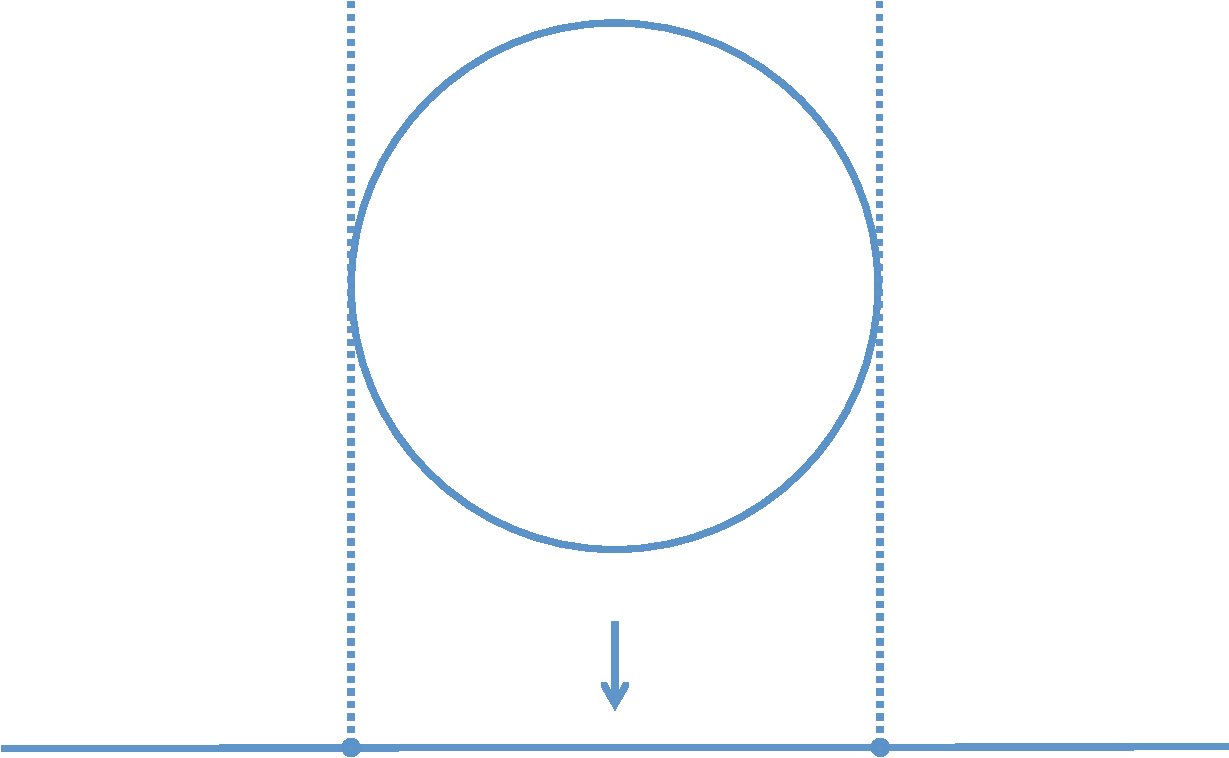
\includegraphics[width=.7\textwidth]{presheaf_1.pdf}
\caption{Cohomology Pre-sheaf is Non-Local}
\label{fig:nonlocal_presheaf}
\end{figure}

\end{ex}


\begin{ex}[Inconsistent]\label{ex:inconsistentpresheaf}\index{presheaf!inconsistent example}
Let $F$ be a presheaf of sets over the real line $\R$, defined as follows:
\begin{equation*}
 F(U)=
\begin{cases}
 \{a,b\} & \text{if } U=X \\
\{\star\} & \text{o.w.}
\end{cases}
\end{equation*}
This presheaf is like two friends that agree on every possible political issue, but still belong to two different political parties.
\end{ex}

Fortunately, there is a general method of repair that can make any presheaf $F$ into a sheaf $\widetilde{F}$. Although this method modifies the value of $F$ on open sets, it leaves at least one feature of the presheaf unchanged. This is the stalk of the presheaf.

\begin{defn}\index{stalk}\index{presheaf!stalk}\index{sheaf!stalk}
Let $F$ be a pre-sheaf on a topological space $X$ and $x\in X$ a point. The \textbf{stalk} of $F$ at $x$ is the direct limit of $F$ over open sets $U$ containing $x$:
\[
F_x:=\varinjlim_{U\ni x} F(U)
\]
The stalk is the ``local value'' of a presheaf at $x$. Notice that every element $t\in F(U)$ with $x\in U$ has an associated value $t_x$, which is the image of $t$ in the direct limit.
\end{defn}
\begin{rmk}
 Since $F$ only assigns data to open sets, one often uses the direct limit construction to assign data to arbitrary sets of $X$; the stalk is just a special example of this principle.
 \end{rmk}

Now we introduce the procedure for turning an arbitrary presheaf of sets, vector spaces or groups into a sheaf of the same type.

\subsubsection{Sheafification}

We begin our introduction to the sheaf associated to a presheaf with a careful introduction to products and disjoint unions, following~\cite{deville2012dynamics}.

\begin{defn}[Disjoint Unions and Products in $\Set$]\index{product}\index{coproduct}\index{disjoint union}
Suppose $\{X_s\}_{s\in S}$ is a family of sets indexed by $S$. The \textbf{disjoint union} is a union that tracks the indexing set:
\[
\bigsqcup_{s\in S} X_s := \bigcup_{s\in S} X_s\times \{s\}
\]
The \textbf{product} can be written as a set of maps:
\[
\prod_{s\in S} X_s := \{ f: S \to \bigsqcup_{s\in S} X_s \,|\, f(s)\in X_s\, \forall s\in S\}
\]
The projection maps 
\[
\pi_{s'}:\prod_{s\in S} X_s \to X_{s'}
\]
are defined by evaluation $\pi_{s'}(f)=f(s')$.
\end{defn}

\begin{defn}[Sheafification]\label{defn:sheafification}\index{sheaf!sheafification}
Let $F:\Open(X)^{op}\to\Set$ be a presheaf of sets and let $F_x$ denote the stalk of $F$ at $x$. Now for each open set $U$, form the product $\prod_{x\in U}F_x$. The \textbf{sheafification} $\widetilde{F}$ of $F$ assigns to every open set $U$ the functions in $\prod_{x\in U}F_x$ that ``locally extend,'' i.e.
\[
\widetilde{F}(U):=\{s\in \prod_{x\in U}F_x\,|\, \forall x\in U\, s(x)\in F_x\,, \exists V\ni x\, V\subset U\,t\in F(V)\,\mathrm{s.t.}\, t_y=s(y)\,\forall y\in V\}
\]
There is a natural transformation $\theta:F\to \widetilde{F}$ that takes every element $s\in F(U)$ to the map $s:x\in U \mapsto s_x\in F_x$. In particular, $\theta_x:F_x\to\widetilde{F}_x$ is an isomorphism.
\end{defn}

One can summarize sheafification more elegantly in the language of categories. Since every sheaf is also a pre-sheaf, we have an inclusion functor
\[
\iota:\Shv(X;\Set)\hookrightarrow \Fun(\Open(X)^{op},\Set)=:\Preshv(X;\Set)
\]
that has a left adjoint, i.e. there is a universal natural transformation $\theta:\id_{\Preshv}\to \iota\circ \widetilde{(-)}$, see Section~\ref{sec:adjunctions} for a reminder. Such a subcategory is called \textbf{reflective}. This guarantees, for example, that if $F$ is an arbitrary pre-sheaf and $G$ is a sheaf regarded as a pre-sheaf $G=\iota(G)$, then we have the following universal property:\index{sheaf!sheafification!universal property as a left adjoint}
\[
\xymatrix{ & \widetilde{F} \ar@{.>}[d]^{\exists !} \\ F \ar[ur]^{\theta_F} \ar[r]^{\varphi} & \iota(G)}
\]
Pulling back along $\theta_F$ induces the natural isomorphism of $\Hom$-sets:
\[
\Hom_{\Shv}(\widetilde{F},G)\cong \Hom_{\Preshv}(F,\iota(G))
\]

\subsection{Grothendieck's Operations}\label{subsec:six_ops}
\index{Grothendieck!Six Functor Formalism}

What makes sheaf theory such a powerful machine is that there are many natural operations on sheaves and well understood adjunctions between these operations. However, many of these operations only exist with the aid of sheafification. In particular, there are the following six operations, grouped into three adjoint pairs, the third of which exists only in a suitable enlargement of the category of sheaves.
\[
(f^*,f_*) \qquad (\otimes,\SHom) \qquad (f_!,f^!)
\]
Here we will consider only four out of the six in order to forego this extra difficulty of ``enlarging'' the category of sheaves.

\begin{defn}[Pushforward Sheaf]\index{sheaf!pushforward}
Let $f:Y\to X$ be a continuous map and let $G$ be a sheaf on $Y$. The \textbf{pushforward sheaf} is defined by the formula:
\[
f_*G(U):=G(f^{-1}(U))
\]
\end{defn}

There should be an inverse operation that takes a sheaf $F$ on $X$ and pulls back along $f:Y\to X$. After all, if $i:W\hookrightarrow X$ is the inclusion of an open set, then a natural candidate for the pullback sheaf $i^*F$ would be the restriction of the domain of definition of $F$ to only those open sets contained in $W$.
\[
F|_W(U)=F(U)
\]
However, if $f:Y\to X$ is not an open map, then there is no hope for an easy definition. Sheafification, however, comes to the rescue.

\begin{defn}[Pullback Sheaf]\index{sheaf!pullback}\index{pullback!of sheaves}
Let $f:Y\to X$ be a continuous map and $F$ a sheaf on $X$. The \textbf{pullback sheaf}, written $f^*F$ is the sheafification of the pre-sheaf
\[
U\rightsquigarrow \varinjlim_{V\supset f(U)} F(V)
\]
\end{defn}

\begin{ex}[The Stalk]\index{stalk}\index{sheaf!stalk}
Let $i:\{x\}\hookrightarrow X$ be the inclusion of a point into a space with a sheaf $F$ defined on it. The sheaf $i^*F\cong F_x$ is the stalk at $x$.
\end{ex}
\begin{exr}
Verify for $i:W\hookrightarrow X$ that $i^*F=F|_W$
\end{exr}

The next pair of interest is the middle pair.
\begin{defn}[Sheaf Hom]\index{sheaf!Hom@$\SHom$}
Suppose $F$ and $G$ are sheaves of abelian groups over a single space $X$. The \textbf{sheaf hom} $\SHom(F,G)$ assigns to every open set
\[
\SHom(F,G)(U):=\Hom_{\Shv(U)}(F|_U,G|_U)
\]
\end{defn}

For the algebraically minded, there should be a knee-jerk response for an associated tensor sheaf, however the na\"ive assignment needs to be sheafified.

\begin{defn}\index{sheaf!tensor@$\otimes$}
Suppose $F$ and $G$ are sheaves of abelian groups over a single space $X$. The \textbf{tensor product of sheaves} $F\otimes G$ is defined to be the sheafification of the assignment
\[
U\rightsquigarrow F(U)\otimes G(U)
\]
\end{defn}

The reader is encouraged to work through the following exercise, borrowed from~\cite{achar-lsu} with a few extra hints.

\begin{exr}
Let $Q$ be the sheaf of sections of the map $f:S^1\to S^1$ defined via complex coordinates as $f(z)=z^2$, i.e.
\[
Q(U):=\{s:U\to S^1\,|\, f\circ s(z)=z\}.
\]
Check that this sheaf has no global sections. Now let $Q_{k}$ be the sheaf which assigns to each open set $U$ the $k$ vector space freely generated by the set $Q(U)$. Show by taking a carefully chosen cover of $S^1$ that
\[
F:U\rightsquigarrow Q_{k}(U)\otimes Q_{k}(U)
\]
is not a sheaf. Observe that we have a natural method for tensoring elements of $Q_{k}(U)$ together via pointwise multiplication. Any element $s\in Q_{k}(U)$ satisfies $(s\otimes s)(z)=s(z)^2=z$, but there are interesting cross-multiple terms.
\end{exr}

Although working out the above exercise is rewarding, the category theorist knows that since tensor products are colimit constructions and the sheaf axiom involves limits, one should instantly be suspicious of such a construction defining a sheaf. However, one can construct cosheaf-theoretic analogs of the above functors and there the tensor cosheaf is naturally a cosheaf, but cosheaf Hom needs to be ``cosheafified,'' if such a thing exists.

\subsection{Failures to Commute}\label{subsec:failure_to_commute}

Unfortunately, the universe appears to have a sort of handedness that makes certain constructions for sheaves natural, but not so for cosheaves. This is because most data categories $\dat$, such as $\Set,\Vect$ or $\Ab$, are not equivalent to their opposite categories. Thus the topological simplification of reducing cosheaves to sheaves comes at the cost of making the algebraic thinking more difficult. In particular, certain properties of $\dat=\Set,\Vect$ or $\Ab$ are used in the development of sheaf theory, which do not necessarily hold in $\dat^{op}$. The centerpiece of this discussion will be understanding that filtered colimits commute with finite limits in $\dat$, but cofiltered limits do not necessarily commute with finite colimits in $\dat$. Let us now relay the necessary definitions.

\begin{defn}\index{category!co@(co)filtered}
	A non-empty category $\cat$ is called \textbf{filtered} if the following two properties are satisfied: 
	\begin{itemize}
		\item For every pair of objects $x, y\in \cat$ there is a third object $z\in \cat$ with $x\to z$ and $y\to z$.
		\item For every pair of parallel morphisms $f,g:x\to y$ there is a third object and morphism $h:y\to z$ such that $h\circ f=h\circ g$.
	\end{itemize}
	A category $\cat$ is called \textbf{cofiltered} if $\cat^{op}$ is filtered. Sometimes, when the category is especially simple, we will simply call a cofiltered category filtered.
\end{defn}

\begin{ex}\index{category!of covers}
In Section~\ref{subsec:refinement} we considered the category of covers $\Cov(U)$ of an open set $U$. By noting that any two covers have a common refinement, one sees that this is an example of a cofiltered (or \emph{cofiltrant}) category.
\end{ex}

\begin{defn}\index{limit!cofiltered}\index{colimit!filtered}
	Suppose $I$ is a filtered indexing category with $F:I\to\dat$ and $G:I^{op}\to\dat$ diagrams in some category. We will call the colimit of $F$ a \textbf{filtered colimit} and the limit of $G$ a \textbf{cofiltered limit}.
\end{defn}

Now we give an example already introduced in the context of sheafification.
\begin{ex}[(Co)Stalks]\index{costalk}\index{stalk}
	Suppose $X$ is a topological space and $x$ is a point in $X$. The set of open sets containing $x$ defines a cofiltered subcategory of $\Open(X)$ or a filtered subcategory of $\Open(X)^{op}$. Consequently for a pre-sheaf $F$ or a pre-cosheaf $\hF$, the following
	\[
	F_x:=\varinjlim_{U\ni x} F(U) \qquad \varprojlim_{U\ni x}\hF(U)=:\hF_x
	\]
	define a filtered colimit and cofiltered limit, respectively. These are called the \textbf{stalk at x} of a pre-sheaf $F$ and the \textbf{costalk at x} of a pre-cosheaf $\hF$. Of course, to make such a statement meaningful, one needs to assume the data category $\dat$ has the relevant limits and colimits.
\end{ex}

The following theorem illustrates one of the fundamental differences between sheaves and cosheaves. It is expressed through the following algebraic fact, which the reader might like to compare with the Fubini theorem.
\begin{thm}\label{thm:filteredcolimits}\index{colimit!filtered!commutes with finite limits}
	Let $I$ be a filtered indexing category and $J$ a finite category. Then any functor $\alpha:I\times J\to\dat$ where $\dat=\Set,\Vect,$ or $\Ab$, has the property that the natural map
	\[
		\varinjlim_I\varprojlim_J \alpha(i,j) \to \varprojlim_J\varinjlim_I \alpha(i,j)
	\]
	is an isomorphism. We say for short that ``filtered colimits and finite limits commute'' in these categories.
\end{thm}
\begin{proof}
For a proof of this statement, we refer the reader to theorem 3.1.6 in~\cite{KS-CS}. First note that the product category $I\times J$ is just a product in $\Cat$ - the category of all categories. We can describe the objects of $I\times J$ as pairs of objects, one from each category, and the morphisms as tuples of morphisms, one for each object. One can take $\alpha$ and then define a new functor $\varprojlim_J \alpha:I\to\dat$ gotten by assigning to each object $i\in\obj(I)$ the limit over $J$ of $\alpha(i,-):J\to\dat$. Taking the colimit over $I$ defines the first expression. Similar reasoning defines the second.
\end{proof}

\index{exact!sequence of presheaves}\index{exact!sequence of sheaves}\index{sheaves!exact sequence of}\index{presheaf!exact sequence}
For an application of this theorem we introduce some ideas to the world of pre-sheaves valued in $\Vect$. Recall that a complex of vector spaces 
\[
\cdots \to V_1\to V_2 \to V_3 \to \cdots
\] 
is exact at a term in a sequence if the image of the incoming map coincides with the kernel of the outgoing map. A sequence of pre-sheaves\footnote{The corresponding statement for sheaves is \emph{not} true.} is exact if and only if for each open set $U$ the associated sequence of vector spaces is exact, i.e.
\[
	0 \to E \to F \to G \to 0 \qquad \mathrm{iff} \qquad 0 \to E(U) \to F(U) \to G(U) \to 0
\]
Theorem~\ref{thm:filteredcolimits} then implies that for any point $x\in X$ the induced sequence of stalks
\[
	0 \to E_x \to F_x \to G_x \to 0
\]
is exact. Intuitively this is because we can view $E$ as a kernel of the pre-sheaf map $F\to G$ and as already demonstrated, kernels are examples of finite limits. Thus taking the kernel of the stalk map $F_x\to G_x$ is the same as taking the stalk of the kernel of $F\to G$.

\begin{prop}\label{prop:dont_commute}\index{limit!cofiltered!do not commute with finite colimits}
	For $\dat=\Set,\Vect$ or $\Ab$ it is not true that cofiltered limits and finite colimits commute. Consequently, if $A,B,C:\NN^{op}\to\Ab$ (or $\Vect$) are functors from the category of natural numbers equipped with the opposite ordering, with natural transformations $A\to B \to C$ such that
	\[
		\xymatrix{ 0 \ar[r] & A_i \ar[r] & B_i \ar[r] & C_i \ar[r] & 0}
	\]
	is exact for every $i$, then it is \emph{not always} the case that the induced sequence on limits is exact.
	\[
		\xymatrix{ 0 \ar[r] & \varprojlim A \ar[r] & \varprojlim B \ar[r] & \varprojlim C \ar[r] & 0}
	\]
\end{prop}
\begin{proof}
	We borrow an example from Jason McCarthy's notes~\cite{limits-jason}. Consider the following system of short exact sequences of groups:
	\[
		\xymatrix{\vdots \ar[d] & \vdots \ar[d] & \vdots \ar[d] & \vdots \ar[d] & \vdots \ar[d] \\
		0 \ar[d] \ar[r] & \ZZ \ar[d]_{n+1} \ar[r]^n & \ZZ \ar[d]_{n+1} \ar[r] & \ZZ/n \ar[r] \ar[d]_{\id} & 0 \ar[d] \\
		0 \ar[d] \ar[r] & \ZZ \ar[d]_{n+1} \ar[r]^n & \ZZ \ar[d]_{n+1} \ar[r] & \ZZ/n \ar[r] \ar[d]_{\id} & 0 \ar[d] \\
		0  \ar[r] & \ZZ  \ar[r]^n & \ZZ  \ar[r] & \ZZ/n \ar[r] & 0}
	\]
	The inverse limit of the first (and second) column with non-zero entries must be zero. To see why, note that the inverse limit can be described as
	\[
		\varprojlim_{\NN^{op}} \ZZ_i = \{(x_i)\in \prod_i \ZZ_i\, |\, x_i=(n+1)^{j-i}x_j \,\forall j\geq i\},
	\]
	where we have viewed the indexing category as the natural numbers with the opposite ordering. Any non-zero element of the limit would have some non-zero factor $x_i$ and consequently all other factors would be non-zero (since the map $a\to (n+1)a$ is injective). In particular, all higher $x_j$ must be equal to $x_i/(n+1)^{j-i}$, but letting $j$ be suitably large would imply that $x_j$ must be less than one --- an impossibility. Thus the induced map of inverse limits is
	\[
		\xymatrix{0 \ar[r] & 0 \ar[r] & 0 \ar[r] & \ZZ/n\ZZ \ar[r] & 0}
	\]
	which is not exact. If the reader prefers an example in the category of vector spaces, one should see Schapira's example 4.2.5 in his notes~\cite{schapira-AlTo}.
\end{proof}

Thus the statement that short exact sequences of pre-cosheaves induces a short exact sequence on costalks cannot be guaranteed. There is a subtle work-around that says under suitable hypotheses\footnote{i.e. the Mittag-Leffler condition. See~\cite[Sec. 1.12]{KS} or~\cite[pp. 211-214]{alpine} for more details.} exactness can be guaranteed. This holds for categories like $\vect$, the category of finite-dimensional vector spaces, and $\mathbf{ab}$, the category of finite abelian groups, because this is where the descending chain condition holds~\cite{atiyah-mac}.


This last comment about $\vect$ provides justification for performing some dualization to obtain results about cosheaves from sheaves. After all, for finite-dimensional vector spaces it is true that
\[
	\Hom_{\vect}(-,k):\vect^{op}\to\vect
\]
establishes an equivalence of categories.\footnote{This does \emph{not} extend to an equivalence between $\Vect$ and its opposite category. In fact, $\Vect^{op}$ is equivalent to the category $\pro-\vect$, cf.~\cite[Rmk.6.2]{isaksen-pro}.\index{category!opposite!of Vect@$\Vect$}} However, issues of stalks versus costalks is not the primary obstacle that the asymmetry of Theorem~\ref{thm:filteredcolimits} presents. That obstacle has to do with a process known as \textbf{sheafification}, which provides a universal tool for turning any pre-sheaf into a sheaf. For most texts on sheaf theory it is presented before almost any other theory is developed.

\index{sheaf!sheafification}
The most general sheafification process outlined by Grothendieck takes a pre-sheaf $F$ and defines a new pre-sheaf $F^+$ that assigns to each open set $U$ the filtered colimit of $F:\Cov(U)^{op}\to\dat$, see~\cite[Sec. 17.4]{KS-CS} for a modern exposition. Applying this construction twice defines a sheaf. However, in order to guarantee that this $F^{++}$ is a sheaf one uses the properties of Theorem~\ref{thm:filteredcolimits}. This now gets us to the more fundamental reason why the study of cosheaves may be so obscure: The non-exactness of $\varprojlim$ thwarts the Grothendieck prescription for cosheafification. \emph{For pre-cosheaves valued in $\Set, \Ab$ or $\Vect$ there is simply no hope in using the standard, most general, cosheafification.}
\index{cosheaf!cosheafification!approaches}

There are a very small handful of approaches that have been used to circumvent this problem:
\begin{enumerate}
 \item \textbf{\v{C}ech Homology and Smoothness}: One approach developed by Bredon~\cite{bredon-ch,Bredon} is to define an equivalence relation on pre-cosheaves, more nuanced than isomorphism, which is constructed through zig-zag diagrams of \emph{local} isomorphisms. Bredon develops an operation which uses \v{C}ech homology to take in one pre-cosheaf and produce another. In the event that the starting pre-cosheaf was equivalent to a cosheaf (Bredon calls such a pre-cosheaf \emph{smooth}), he proves that his construction yields a cosheaf.

 \item \textbf{Pro-Objects}: Another notable approach is to use pro-objects, i.e. functors $P:I^{op}\to\cat$ where $I$ is filtrant. This theory is engineered in such a way that all the desired algebraic properties exist. This approach was perhaps first used by Jean-Pierre Schneiders~\cite{schneiders-ch} to develop a rich theory of cosheaves. The problem with pro-objects is its conceptual and algebraic difficulty. For the visually minded, cosheaves of pro-objects are infinite diagrams of infinite diagrams, which obscure the many natural examples of pre-cosheaves and cosheaves that one might want to capture. More recent work~\cite{sugiki,prasolov}, has also used this setup for cosheaves.

 \item \textbf{Topology:} Here, one eschews full generality and works only with certain cosheaves known as \textbf{constructible cosheaves}, which can be thought of as cosheaves on particular finite spaces. Cosheafification in this setting exists and is natural. Often one does not even think about needing to cosheafify, because the diagrams are modeled on the points of the space. This school of thought, motivated by the vision and unpublished ideas of Bob MacPherson, has some recent trace in the literature, see~\cite{woolf, dt-lag}.
\end{enumerate}

For the most part, we choose to sidestep the issues of sheafification and cosheafification by focusing on the third approach. We believe that this provides a better way of learning sheaf theory as it removes the ever-present phrase ``let \emph{blank} be the sheafification of \emph{blank}'' and focuses on the more important technical machinery first. However, we provide a proof that cosheafification does exist in the next section.

\subsection{The Existence of Cosheafification}
\label{subsec:cosheafification}
\index{cosheaf!cosheafification}

Grothendieck gave us a general construction of the sheafification functor $\widetilde{(-)}$ that works in more general data categories $\dat$, which comes from applying a certain functor $(-)^{+}$ twice. The requirement on the category $\dat$ includes, among other things, that filtered colimits and finite limits commute. If we were to regard a pre-cosheaf $\hF:\Open(X)\to\dat$ as a pre-sheaf valued in $\dat^{op}$, then the condition that filtered colimits and finite limits commute in $\dat^{op}$ would become the condition that cofiltered limits and finite colimits commute in $\dat$, which is patently false when $\dat=\Set,\Vect$ or $\Ab$, as the example in Proposition~\ref{prop:dont_commute} showed.

Consequently, we do not have a clear answer to the question: Does the inclusion functor $\iota$ have a \emph{right} adjoint $(-)_{\#}$?\index{cosheaf!cosheafification!universal property as a right adjoint}
\[
\iota:\Coshv(X;\dat) \hookrightarrow \Fun(\Open(X),\dat)=:\Precoshv(X;\dat)
\]
so that the dual universal property is satisfied, i.e. if $\hF$ is a pre-cosheaf and $\hG$ is a cosheaf with a morphism $\hG\to\hF$, then there is a unique way of completing the diagram.
\[
\xymatrix{ & \hF_{\#} \ar[d] \\
\hG \ar@{.>}[ur] \ar[r] & \hF}
\]
\index{cosheaf!cosheafification!exists for Set@$\Set$}
In the case where $\dat=\Set$, Jon Woolf's paper~\cite{woolf} contains a construction of cosheafification. Unfortunately, this cannot be adapted to categories like $\Vect$ or $\Ab$. For a high-level reason why, Mac Lane and Moerdijk explain on page 95 of~\cite{mm-topos} that a sheaf of abelian groups can be identified with an abelian group object in the category of sheaves. Since sheafification preserves finite products, sheafification of pre-sheaves of sets lifts to a functor between abelian group objects. Moreover, since the forgetful functor $for:\Ab\to\Set$ preserves limits (but not colimits), any sheaf of groups defines a sheaf of sets. Trying to repeat this last line of reasoning for cosheaves of groups fails, i.e. a cosheaf of groups does not, by forgetting, define a cosheaf of sets.

Our approach is to verify abstractly whether cosheafification exists without constructing it. Of course, one would like to use Freyd's Adjoint Functor Theorem~\ref{thm:freyd}, but we will use a different theorem~\cite[Thm 6.28]{adamek-lpac} that is easier to check.

\begin{thm}\index{Vopenka's principle}
Assuming Vopenka's principle (a large cardinal axiom), every full subcategory $\bat$ of a locally presentable category $\cat$, where $\bat$ is closed under colimits, is coreflective, i.e. the inclusion functor $\iota:\bat\hookrightarrow\cat$ has a right adjoint (a cofree functor).
\end{thm}

We will leave Vopenka's principle as a black box and assume it, even though many category theorists cringe at its very name. We prove that cosheafification exists by verifying the hypotheses of the above theorem for our case of interest.

\begin{cor}
The category of cosheaves of vector spaces is a coreflective subcategory of $\Fun(\Open(X),\Vect)$, i.e. cosheafification exists.
\end{cor}
\begin{proof}
It is clear that the category of cosheaves is closed under colimits, since we can define the colimit to be the pre-cosheaf, which open-by-open assigns the colimit of vector spaces over that open set. This pre-cosheaf is a cosheaf, because for a fixed cover, each vector space in the diagram is expressed as a colimit and colimits commute with colimits.

It remains to be seen that the category of pre-cosheaves is locally presentable. this means that the category is locally small, has small colimits, has a small set of objects $\covS$ that generates $\Precoshv(X;\Vect)$ in the sense that every pre-cosheaf is a colimit of objects in $\covS$, and every object is small. The first two statements are easily addressed. $\Open(X)$ is a small category and $\Vect$ is locally small, so the functor category is locally small. Colimits of pre-cosheaves are defined open-by-open. Since $\Vect$ is cocomplete, pre-cosheaves valued in $\Vect$ is also cocomplete. Now we address the existence of a generating set. 

Define, for each open set $U\in \Open(X)$, the following pre-cosheaf:
\[
\hat{h}_U(V)=\left\{\begin{array}{ll} k & if\, U\subset V \\ 0 & o.w.\end{array}\right.
\]
We'd like to say that every pre-cosheaf is a colimit of pre-cosheaves of the above form. The corresponding statement for pre-sheaves is proved in pages 41-42 of~\cite{mm-topos}. We will go ahead and repeat the argument here. Note that if $\hG$ is an arbitrary pre-cosheaf, then
\[
\Hom_{\Precoshv}(\hat{h}_U,\hG)\cong \hG(U).
\]
Observe that if $U\subset U'$, then we get a map of pre-cosheaves (a natural transformation) $\hat{h}_{U'}\to \hat{h}_{U}$. This in turn induces a map
\[
\Hom_{\Precoshv}(\hat{h}_U,\hG)\to \Hom_{\Precoshv}(\hat{h}_{U'},\hG)
\]
which coincides with the internal extension map of $\hG$, that is $r_{U',U}:\hG(U)\to \hG(U')$. In other words, the functor
\[
R:\Precoshv(X;\Vect)\to\Precoshv(X;\Vect)
\] 
\[
G \rightsquigarrow (U\mapsto \Hom_{\Precoshv}(\hat{h}_U,\hG)\cong \hG(U))
\]
is isomorphic to the identity functor. Since adjoints are unique up to isomorphism, then we can conclude that its (left) adjoint must also be isomorphic to the identity functor. However, we will construct explicitly the adjoint, which, combined with the fact that it must be the identity functor, exhibits $\hG$ as the colimit of pre-cosheaves of the form $\hat{h}_U$.

For each pre-cosheaf $\hG$, define the following \textbf{category of elements} $J_{\hG}$.\footnote{It should be noted that in~\cite{mm-topos}, the category of elements is written $\int \hG$.} The objects of $J_{\hG}$ are pairs
\[
(U,x) \qquad \mathrm{where} \qquad U\in\Open(X) \quad x\in \hG(U).
\]
A morphism $(U,x)\to (U',x')$ is defined if $U\subset U'$ and $x'=r_{U',U}(x)$. Clearly, there is a projection functor $\pi_{\hG}:J_{\hG}\to\Open(X)$ and by formality, there is a dual functor $\pi^{op}_{\hG}:J_{\hG}^{op}\to\Open(X)^{op}$.

Denote by $\mathcal{Y}$ the functor
\[
\mathcal{Y}:\Open(X)^{op}\to\Precoshv(X;\Vect) \qquad \qquad U \rightsquigarrow \hat{h}_U.
\]
We claim that the left adjoint $L$ to the functor $R$ considered above can be constructed object-wise as follows: for each pre-cosheaf $\hG$ define
\[
L(\hG):=\varinjlim \mathcal{Y}\circ \pi_{\hG}^{op}.
\]
We claim that $\hG$ is the colimit. This is already given from the fact that $L$ must be isomorphic to the identity functor, but let's at least check how $\hG$ is a co-cone, to make the statement more plausible. For each object $(U,x)$ in $J_{\hG}$ the map to $\hG$ is defined by
\[
x\in \hG(U)\cong \Hom_{\Precoshv}(\hat{h}_U,\hG)\ni \psi_{U,x}
\]
where $\psi_{U,x}$ is the natural transformation that sends $1\in\hat{h}_U(U)$ to $x\in \hG(U)$ and then for any larger open set $U\subset U'$ sends $1\in\hat{h}_U(U')$ to $r_{U',U}(x)$.
Observe that if $U\subset U'$ and $(U',x')\to (U,x)$ is a morphism in $J_{\hG}^{op}$, so $r_{U',U}(x)=x'$, then we have the following commutative diagram:
\[
\xymatrix{(U',x')\ar[d] \ar@{~>}[r] & \hat{h}_{U'}\ar[d] \ar[rd]^{\psi_{U,x'}} & \\
(U,x) \ar@{~>}[r] & \hat{h}_{U} \ar[r]_{\psi_{U,x}} & \hG}
\]
At the risk of demonstrating the obvious, the above diagram commutes if the the following diagram commutes for an arbitrary triple of open sets $V\subset V'\subset V''$. We will check it for the interesting boundary case $U\subset U'\subset U''$.
\[
\xymatrix{\hat{h}_{U'}(U'')=k \ar[r]^1 & \hat{h}_{U}(U'')=k \ar[r]^{r_{U'',U'}(x)} & \hG(U'') \\
\hat{h}_{U'}(U')=k \ar[r]^1 \ar[u]^1 & \hat{h}_U(U')=k \ar[u]^1 \ar[r]^{r_{U,U'}(x)=x'} & \hG(U') \ar[u]_{r_{U'',U'}} \\
\hat{h}_{u'}(U)=0 \ar[r] \ar[u] & \hat{h}_U(U)=k \ar[r]^{x} \ar[u]^1 & \hG(U) \ar[u]_{r_{U',U}} }
\]
This completes the plausibility check. We use the observation that $L$ is isomorphic to the identity functor to conclude that $\hG$ is actually the colimit. The conclusion is that
\[
\hG\cong \varinjlim \mathcal{Y}\circ\pi_{\hG}^{op}
\]
i.e. $\hG$ is expressible as a small colimit of pre-cosheaves of the form $\hat{h}_U$ where the size of the indexing set is bounded by the product of the cardinality of $\Open(X)$ and the maximum cardinality of $\hG(U)$ over varying $U$.

Now it remains to check the smallness of objects in $\Precoshv(X;\Vect)$. An object $\hG$ is small if there exists a regular cardinal $\kappa$ such that $\Hom(\hG,-)$ commutes with directed colimits of diagrams indexed by categories of cardinality at most $\kappa$.

Observe that for one of our pre-cosheaves $\hat{h}_U$ is compact since if $(\hF_i)$ is a direct system of pre-cosheaves, then
\[
\varinjlim\Hom(\hat{h}_U,\hF_i)\cong \varinjlim \hF_i \cong \Hom(\hat{h}_U,\varinjlim \hF_i).
\]
As already shown, for every pre-cosheaf $\hG$ there exists a diagram whose cardinality is the cardinality of $J_{\hG}$, which we will call $\kappa_J$. Now, we know how to express $\hG$ as a colimit of $\hat{h}_U$'s. Thus,
\begin{eqnarray*}
\Hom(\hG,\varinjlim_i \hF_i) &\cong & \Hom(\varinjlim_U \hat{h}_U,\varinjlim_i \hF_i)\\
&\cong &\varprojlim_U \Hom(\hat{h}_U,\varprojlim_i \hF_i) \\
&\cong &\varprojlim_U\varinjlim_i \Hom(\hat{h}_U,\hF_i) \\
&\cong &\varprojlim_i\varinjlim_U \Hom(\hat{h}_U,\hF_i) \\
&\cong &\varinjlim_i\Hom(\varinjlim_U \hat{h}_U,\hF_i) \\
&\cong &\varinjlim_i\Hom(\hG,\hF_i)
\end{eqnarray*}

The third line follows from compactness of $\hat{h}_U$. The fourth line follows from the fact that in $\Set$, $\kappa_J$ small colimits commute with $\kappa_J$ -filtered colimits. This completes the proof.

\end{proof}